\chapter{Sprint 1 -- Discovery and Data Model Mapping}

% ---------------------------------------------------------
\section*{Introduction}
\addcontentsline{toc}{section}{Introduction}
% ---------------------------------------------------------

\paragraph{}This chapter presents the first sprint of the project, which spanned two weeks. Its purpose was not to
implement the generator yet, but to clarify the financial and technical rules needed before
implementation. Since the application produces data for Longview, the sprint identified the meaning
of the main entities to generate, their dependencies, and the constraints that must be respected by
the later SQL generation pipeline.


% ---------------------------------------------------------
\section{Sprint Backlog}
% ---------------------------------------------------------

\paragraph{}Sprint 1 targeted user story \textbf{US-1}, dedicated to discovering and documenting the
Longview data model before starting the generation engine. The sprint backlog is presented in
Table~\ref{tab:sprint1-backlog}.

\Needspace{12\baselineskip}
\renewcommand{\arraystretch}{1.35}
\begin{longtable}{|Q{0.08\textwidth}|P{0.28\textwidth}|P{0.42\textwidth}|Q{0.12\textwidth}|}
\caption{Sprint 1 backlog}
\label{tab:sprint1-backlog} \\
\hline
\textbf{ID} & \textbf{Task} & \textbf{Description} & \textbf{Estimate} \\
\hline
\endfirsthead
\multicolumn{4}{r}{\tablename\ \thetable{} -- \textit{continued from previous page}} \\
\hline
\textbf{ID} & \textbf{Task} & \textbf{Description} & \textbf{Estimate} \\
\hline
\endhead
\hline
\multicolumn{4}{r}{\textit{continued on next page}} \\
\endfoot
\hline
\endlastfoot
T1-1 & Review existing SQL and extract files & Identify the files used by the QA team, the tables they populate, and the business entities behind them. & 2 days \\
\hline
T1-2 & Study pre-BCP buffer tables & Document the columns, mandatory fields, keys, and identity columns required by the Longview loading layer. & 3 days \\
\hline
T1-3 & Map stored procedures and load order & Identify the loading procedures and the dependency order that must be respected when generating SQL. & 2 days \\
\hline
T1-4 & Extract business rules & Collect the main financial constraints, code lists, and referential rules used to validate the generated records. & 2 days \\
\hline
T1-5 & Produce entity diagrams & Consolidate the discovered entities, attributes, and relationships into UML class diagrams. & 1 day \\
\end{longtable}

% ---------------------------------------------------------
\section{Sprint Specification}
% ---------------------------------------------------------

\paragraph{}The specification work of Sprint 1 transformed existing Longview material into a clear
generation scope. The sprint identified which business entities had to be generated, how they depend
on each other, and which rules must be preserved by the later generation engine.

\subsection{Target Entity Scope}

\paragraph{}Since Longview contains many extract files, Sprint 1 first reduced the scope to the data
most useful for QA scenarios. Existing extract files, manually written SQL scripts, and QA feedback
were analyzed to identify the entities that are frequently needed, strongly dependent on each other,
and difficult to create manually. The selected scope covers accounts and account groups, models,
securities, prices, hierarchy rows, positions, proposed orders, orders, and executions.

\subsection{Financial Concept Mapping}

\paragraph{}The selected extracts were mapped to the main financial concepts needed by QA
scenarios. This mapping, summarized in Table~\ref{tab:finance-map}, helped separate the business
meaning of each entity from its role in the generator.

\Needspace{10\baselineskip}
\renewcommand{\arraystretch}{1.3}
\begin{longtable}{|P{0.22\textwidth}|P{0.34\textwidth}|P{0.34\textwidth}|}
\caption{Reader's map of the main financial concepts}
\label{tab:finance-map} \\
\hline
\textbf{Concept} & \textbf{Finance meaning} & \textbf{Role in the generator} \\
\hline
\endfirsthead
\multicolumn{3}{r}{\tablename\ \thetable{} -- \textit{continued from previous page}} \\
\hline
\textbf{Concept} & \textbf{Finance meaning} & \textbf{Role in the generator} \\
\hline
\endhead
\hline
\multicolumn{3}{r}{\textit{continued on next page}} \\
\endfoot
\hline
\endlastfoot
Account & A client portfolio or investment account. & Main owner of positions, proposed orders, orders, and optional executions. \\
\hline
Account Group & A business grouping of accounts. & Adds hierarchy and reporting structure around generated accounts. \\
\hline
Model & A target allocation strategy. & Provides allocation data and optional model references for account scenarios. \\
\hline
Security & A tradeable financial instrument such as an equity, bond, option, future, generic instrument, or FX forward. & Central reference reused by prices, hierarchy rows, positions, orders, and executions. \\
\hline
Price & The market value of a security. & Allows generated securities to be valued by Longview. \\
\hline
Position & What an account already owns. & Gives the generator holding context, especially for sell-side order scenarios. \\
\hline
Proposed Order / Order & An intention to trade and the actual trading instruction. & Creates trading activity for valid account-security pairs. \\
\hline
Execution & A market fill confirming that a trade was executed. & Completes the trade lifecycle for generated equity orders. \\
\hline
\end{longtable}

% ---------------------------------------------------------
\subsection{Entity Relationships}
% ---------------------------------------------------------

\paragraph{}After selecting the target extracts, Sprint 1 mapped the relationships required for valid
generation. Prices must reference securities, positions must connect accounts with securities, and
orders must reuse valid account-security pairs. Additional generation rules were also identified, such
as linking options to an underlying security and producing executions from equity orders. This mapping
became the basis for the DTO design and for the later generation pipeline, where services share
generated identifiers instead of producing each output independently.

% ---------------------------------------------------------
\section{Sprint Design}
% ---------------------------------------------------------

\paragraph{}After the sprint specification defined the target entities and their relationships, the
design work focused on how these entities must be loaded by Longview. This design step produced
the pre-BCP loading model, the technical population order, and the UML diagrams used as reference
models for the following sprints.

\subsection{Longview Pre-BCP Loading Mechanism}

\paragraph{}Sprint 1 also clarified the Longview loading mechanism. Generated records are first
inserted into pre-BCP buffer tables, then Longview stored procedures validate them, apply business
rules, and transfer the accepted data into the live schema. Therefore, the generated SQL must target
the buffer tables and respect the required population order, so each referenced account, security,
model, or classification level exists before it is used.

% ---------------------------------------------------------
\subsection{Table Population Order}
% ---------------------------------------------------------

\paragraph{}After understanding the pre-BCP mechanism, the next step was to determine the order
in which the application must write the generated records. This order is used by the SQL script
generator when it emits \texttt{INSERT} statements, identity-column handling blocks, and stored
procedure calls.

\paragraph{}Table~\ref{tab:population-order} summarizes the selected pre-BCP loading order used
by the application. It follows the technical dependency sequence required by Longview.

\Needspace{14\baselineskip}
\renewcommand{\arraystretch}{1.3}
\begin{longtable}{|Q{0.08\textwidth}|P{0.40\textwidth}|P{0.42\textwidth}|}
\caption{Pre-BCP buffer table population order}
\label{tab:population-order} \\
\hline
\textbf{Step} & \textbf{Entity} & \textbf{Dependency} \\
\hline
\endfirsthead
\multicolumn{3}{r}{\tablename\ \thetable{} -- \textit{continued from previous page}} \\
\hline
\textbf{Step} & \textbf{Entity} & \textbf{Dependency} \\
\hline
\endhead
\hline
\multicolumn{3}{r}{\textit{continued on next page}} \\
\endfoot
\hline
\endlastfoot
1 & Security masters: Equity, Fixed Income, Future, Generic and FX Forward & Base security universe. \\
\hline
2 & Option security & Generated after equities and futures because options need an underlying security. \\
\hline
3 & Fixed-income schedules: CALL,PUT,COUP,CONVERT & Fixed income parent security. \\
\hline
4 & Hierarchy & Generated securities and classification definitions. \\
\hline
5 & Price & Security identifiers, including synthetic FX forward identifiers. \\
\hline
6 & Model properties & Generated model names used by model allocations and optional account references. \\
\hline
7 & Model allocations  & Model names from the generated model property records. \\
\hline
8 & Model of Models & Existing parent and submodel identifiers. \\
\hline
9 & Account & No mandatory generated dependency; optional references must already exist when populated. \\
\hline
10 & Account Group & Account membership through \textbf{client\_account\_id}. \\
\hline
11 & Position & Account and security. Generated before orders to support coherent sell scenarios. \\
\hline
12 & Proposed Order & Account, security, and current position context. \\
\hline
13 & Order & Same row shape as proposed orders, loaded with the appropriate Longview procedure mode. \\
\hline
14 & Execution  & Generated from equity orders only; references security and account when supplied. \\
\hline
\end{longtable}

\paragraph{}This order differs from the explanatory business sequence because the SQL script must
satisfy Longview dependencies. The generator therefore creates a coherent business scenario while
emitting SQL in the order accepted by the pre-BCP pipeline.

% ---------------------------------------------------------
\subsection{Entity Class Diagrams}
% ---------------------------------------------------------

\paragraph{}Figure~\ref{fig:class-diagram} presents the UML class diagram produced at the end of
Sprint 1. It served as the reference for the DTO classes and for the generation services implemented
in the following sprint.

\begin{figure}[H]
\centering
\makebox[\textwidth][c]{%
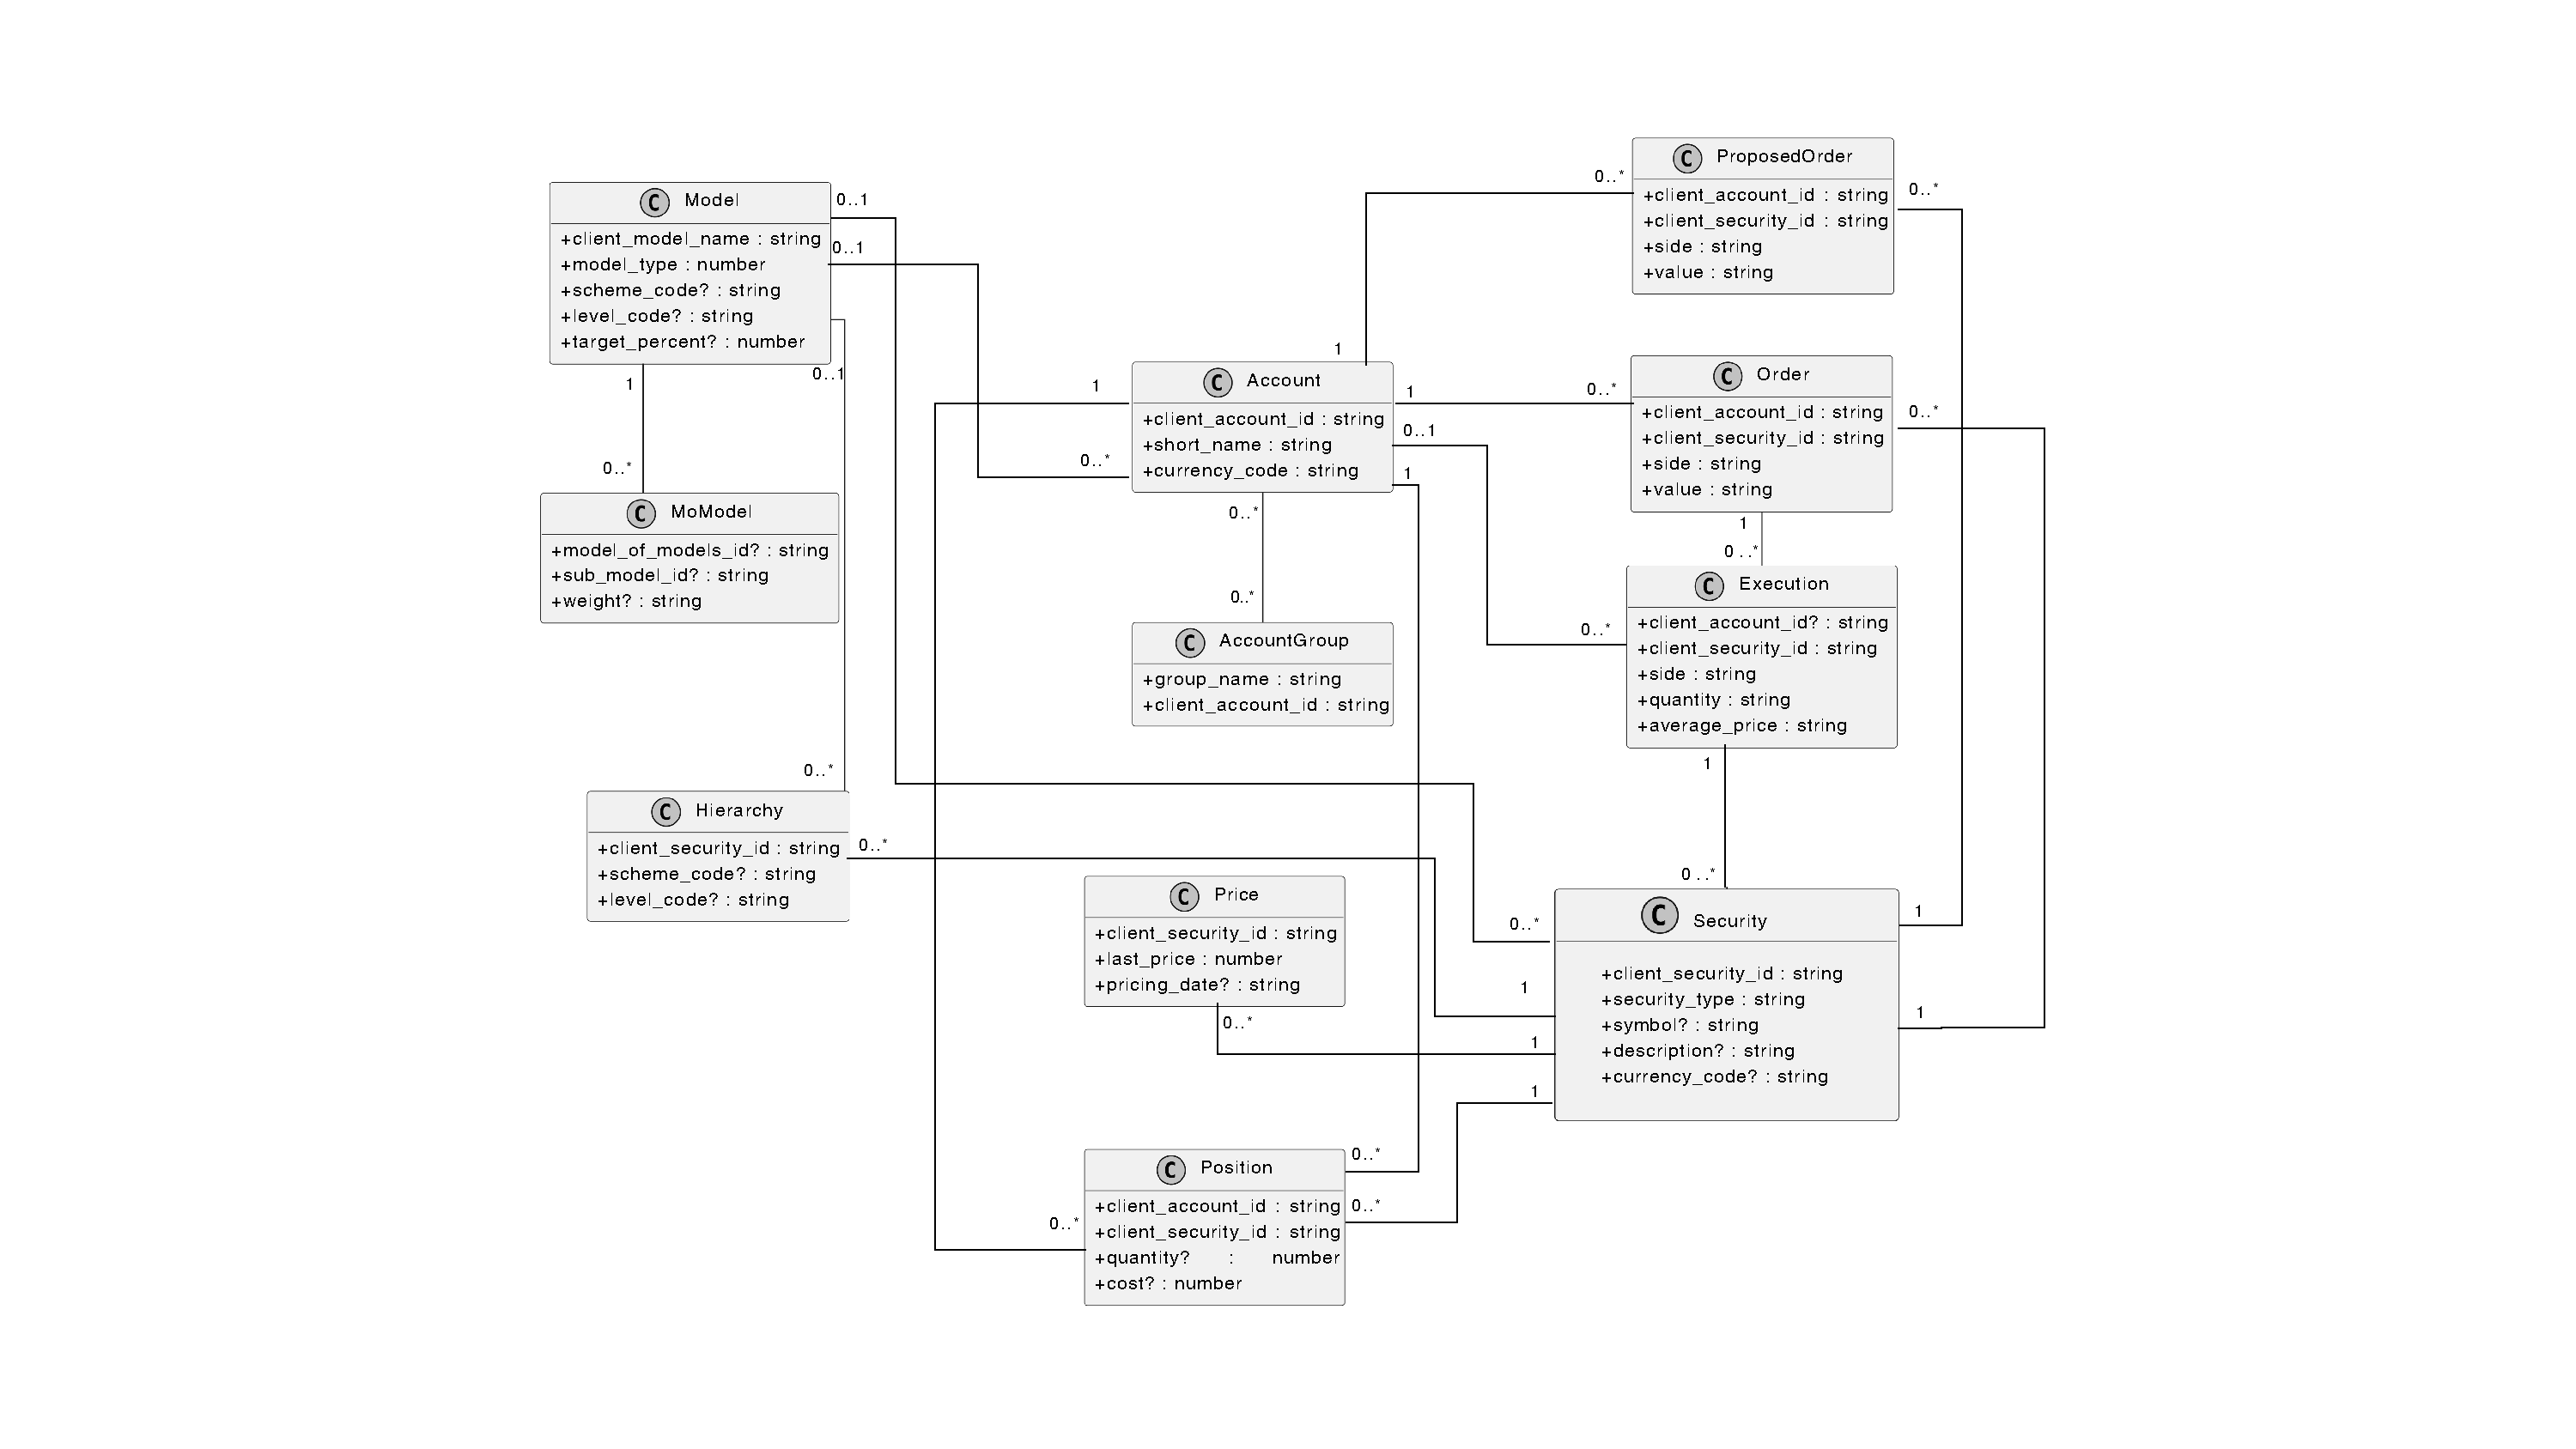
\includegraphics[width=1.5\textwidth,height=0.78\textheight,keepaspectratio]{img/classdiagram-entities.pdf}%
}
\caption{UML class diagram of the Longview entities targeted by the test data generator}
\label{fig:class-diagram}
\end{figure}

\paragraph{}Because securities are the most specialized part of the model, Figure~\ref{fig:security-class-diagram}
isolates the security DTO hierarchy. This separation was needed because each subtype has its own
fields and validation rules.

\begin{figure}[H]
\centering
\makebox[\textwidth][c]{%
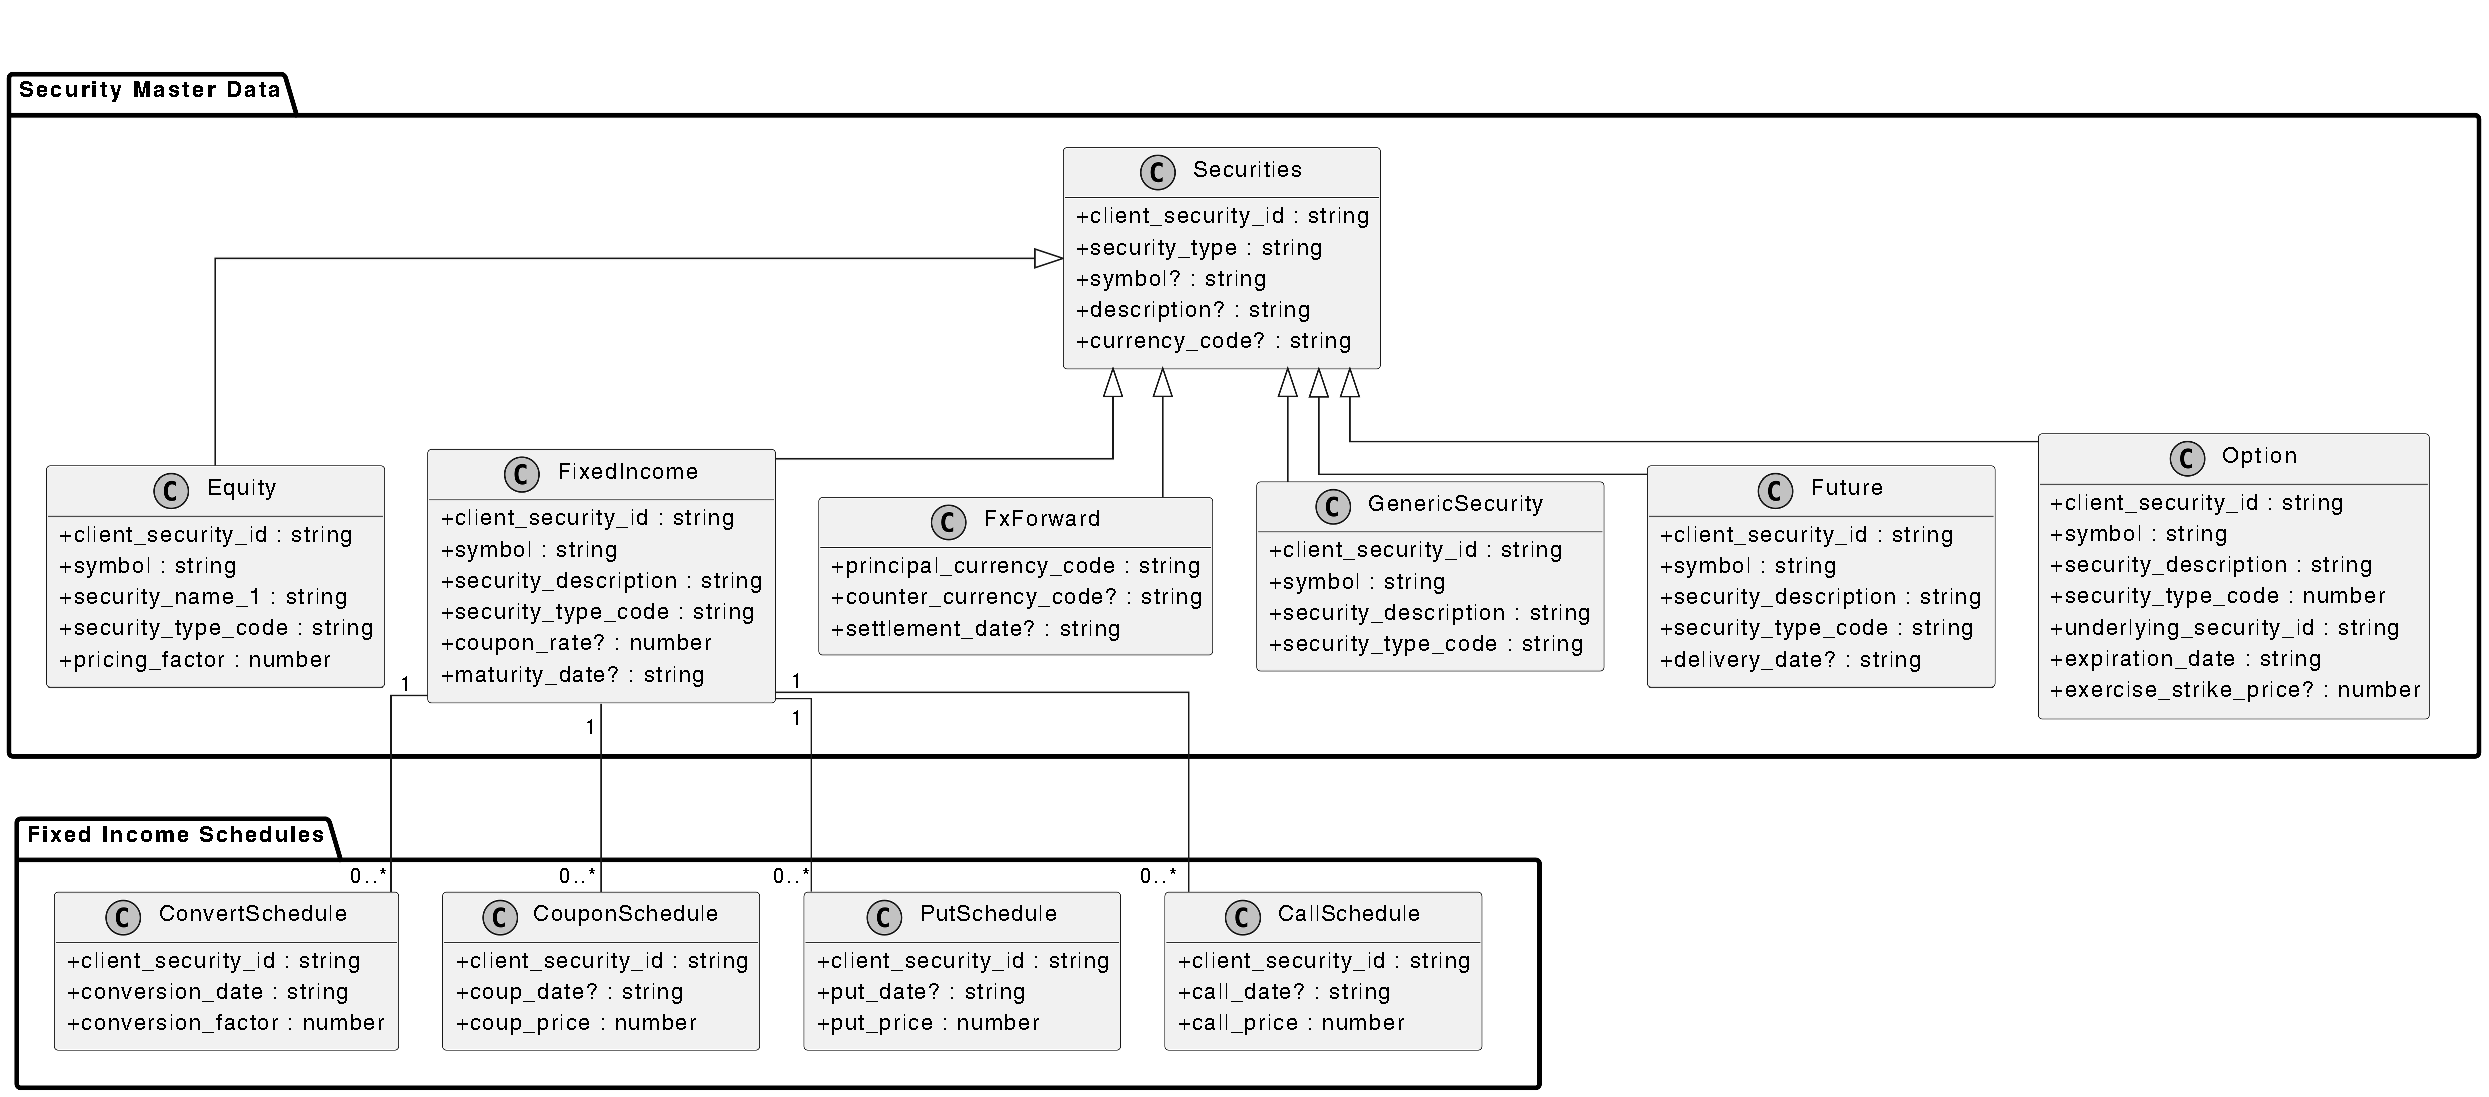
\includegraphics[width=1\textwidth,height=0.78\textheight,keepaspectratio]{img/classdiagram-securities.pdf}%
}
\caption{UML class diagram of the security DTO hierarchy}
\label{fig:security-class-diagram}
\end{figure}

% ---------------------------------------------------------
\section{Realization}
% ---------------------------------------------------------

\paragraph{}The realization of Sprint 1 produced the reference material used before implementation:
the selected entity scope, the relationship rules, the pre-BCP population order, and the UML class
diagrams. The main practical outcome was the separation between the business scenario to generate
and the technical order required by Longview.

\paragraph{}Table~\ref{tab:sprint1-deliverables} summarizes the concrete deliverables produced at
the end of the sprint and explains how each one was reused during the following implementation
sprints.

\Needspace{12\baselineskip}
\renewcommand{\arraystretch}{1.3}
\begin{longtable}{|P{0.28\textwidth}|P{0.31\textwidth}|P{0.31\textwidth}|}
\caption{Sprint 1 realization deliverables}
\label{tab:sprint1-deliverables} \\
\hline
\textbf{Deliverable} & \textbf{Produced result} & \textbf{Use in the project} \\
\hline
\endfirsthead
\multicolumn{3}{r}{\tablename\ \thetable{} -- \textit{continued from previous page}} \\
\hline
\textbf{Deliverable} & \textbf{Produced result} & \textbf{Use in the project} \\
\hline
\endhead
\hline
\multicolumn{3}{r}{\textit{continued on next page}} \\
\endfoot
\hline
\endlastfoot
Selected extracts & Accounts, account groups, models, securities, prices, positions, proposed orders, orders, and executions were selected as the initial generation scope. & Defined the functional perimeter of the standalone generator. \\
\hline
Entity mapping & Each selected business concept was linked to its corresponding DTO, extract file, and pre-BCP buffer table. & Guided the backend DTO structure and generation services. \\
\hline
Relationship rules & Mandatory and optional references between accounts, securities, prices, positions, orders, executions, and models were identified. & Used later by the relationship validation layer. \\
\hline
Population order & The technical loading sequence of the pre-BCP files was established. & Used by the SQL script generation step to emit loadable data in the correct order. \\
\hline
Class diagrams & Entity and security DTO diagrams were produced. & Served as the modeling reference for the implementation of the generation engine. \\
\hline
\end{longtable}
\renewcommand{\arraystretch}{1}

\paragraph{}A screenshot of the analyzed extract folder or an annotated mapping sheet can be added
later in Figure~\ref{fig:sprint1-extract-analysis-proof} to visually document the discovery work
performed during this sprint.

\begin{figure}[H]
\centering
\IfFileExists{img/ch3-extract-analysis-proof.png}{%
    \includegraphics[width=0.88\textwidth]{img/ch3-extract-analysis-proof.png}%
}{%
    \fbox{\parbox[c][0.22\textheight][c]{0.86\textwidth}{\centering Screenshot to be added: selected extracts, mapping sheet, or analyzed SQL files}}%
}
\caption{Sprint 1 extract analysis and mapping evidence}
\label{fig:sprint1-extract-analysis-proof}
\end{figure}

% ---------------------------------------------------------
\section*{Conclusion}
\addcontentsline{toc}{section}{Conclusion}
% ---------------------------------------------------------

\paragraph{}This chapter presented Sprint 1 as the discovery phase that defined the entities,
relationships, loading order, and UML reference models needed before implementation. This
foundation gave Sprint 2 the specification required to build the standalone generation engine and
produce SQL scripts that respect Longview's loading constraints.
